


\section{Evaluation and Discussion}
\label{sec:evaluation}
We evaluate SSDTrain and answer the following questions: 
\begin{enumerate}[Q1.]
\item How well does SSDTrain hide the I/O latency?
\item How much does SSDTrain reduce peak memory usage?
\item How \kwc{does SSDTrain effects translate into advantages as a design choice?}
\end{enumerate}

Section~\ref{sec:exp_baseline} answers Q1 and Q2 by comparing SSDTrain with execution without SSDTrain. \kwc{To answer Q3, w}e \kwc{examine the design space in Section~\ref{sec:exp_dse} and} discuss \kwc{various implications in multiple aspects} in Section~\ref{sec:discussion}.



\subsection{Experimental Setup}
\label{sec:eval_method}
We use a machine with two A100 PCIe GPUs and seven Intel P5800X SSDs, as Table~\ref{tab:configurations} specifies. The SSDs are organized into two RAID0 arrays: one with three SSDs and the other with four SSDs. Each array is the dedicated offloading target of one of the A100 GPUs. We measured the memory usage of the A100 with four SSDs during the evaluation. For consistent performance, the GPUs are locked at base frequency. The latest Megatron-DeepSpeed~\cite{microsoftMicrosoftMegatronDeepSpeedOngoing2019} is installed, incorporating DeepSpeed techniques into Megatron and ensuring interoperability.


\begin{table}[!bhtp]
\centering
\begin{tabular}{rl}
    \toprule
    \textbf{CPU} & 2$\times$ AMD EPYC 7702 64-core\\\cline{1-1}
    \textbf{Memory} & DDR4-3200 1 TB\\\cline{1-1}
    \textbf{GPU} & 2$\times$ Nvidia A100 40 GB PCIe with NVLink \\\cline{1-1}
    \textbf{SSD} & 7$\times$ Intel Optane P5800X 1.6 TB. Two RAID0 arrays. \\\cline{1-1}    \textbf{Software} &     \begin{tabular}[c]{@{}l@{}}Ubuntu 20.04.6~(kernel 5.15.0-113), CUDA 12.2~(driver\\535.183.01), PyTorch 2.2.2, DeepSpeed 0.14.2, Megatron-\\ DeepSpeed~\cite{microsoftMicrosoftMegatronDeepSpeedOngoing2019}~(latest), kvikio 24.08\end{tabular} \\
\bottomrule
\end{tabular}
\caption{Evaluation system configuration.}\label{tab:configurations}
\end{table}

We measure the system pretraining performance on three models: BERT~\cite{devlinBERTPretrainingDeep2019} as an encoder-only model, GPT~\cite{radfordLanguageModelsAre2019} as a decoder-only model, and T5~\cite{raffelExploringLimitsTransfer2023} as an encoder-decoder model. 
We use the OSCAR corpus~\cite{ortiz-suarez-etal-2020-monolingual,OrtizSuarezSagotRomary2019} as the dataset.

\kwc{Before we further explain the model setup, we clarify the batch taxonomy. Like other deep learning models, LLM model training typically uses mini-batches, smaller subsets of the training data. Before Section~\ref{sec:evaluation}, we use the terms ``mini-batch'' and ``batch'' interchangeably.

However, the introduction of data parallelism complicates this terminology: Now, the samples processed in each training step are partitioned into several groups, and each group is assigned to a data-parallel rank. To avoid confusion, in cases where data parallelism is enabled, we refer to all the samples in each training step as a \textit{global batch}, and we refer to the samples assigned to one data-parallel rank a \textit{mini-batch}. Such cases where data parallelism is enabled are only in Section~\ref{sec:discussion}.

Micro-batch is at the lowest level of the batch taxonomy. When gradient accumulation is enabled, a global batch or a mini-batch is further divided into smaller groups for concurrent processing. Similarly, when pipeline parallelism is enabled, such a phenomenon may occur. Each group of samples is called a \textit{micro-batch}. In particular, micro-batch refers to the samples processed in one operator kernel launch.}

We use the two A100 GPUs for tensor parallelism.  The number of micro-batches per step is fixed at one because without pipeline parallelism, in each training iteration, Megatron-DeepSpeed will not start a new micro-batch before both forward propagation and backward propagation of the previous micro-batch are done. A micro-batch number larger than one only brings in gradient accumulation and does not affect the activation offloading pattern. \kwc{In other words, unless stated otherwise, the micro-batch size is equivalent to global batch size throughout Section~\ref{sec:evaluation}.}
\kwc{Throughout Section~\ref{sec:evaluation}, no ZeRO technique is used. Besides, the optimizer states, i.e., what stage-1 ZeRO shards only, may be shared across other dimensions than across the data-parallel ranks: In Megatron or Megatron-DeepSpeed, this is enabled by the \texttt{--use-distributed-optimizer} argument, which we also do not enable in experiments across Section~\ref{sec:evaluation}.}
In our experiments, the hidden dimension is from 8,192 to 16,384, and we use typical hyper-parameters~\cite{devlinBERTPretrainingDeep2019,touvronLlamaOpenFoundation2023,raffelExploringLimitsTransfer2023} for hidden dimensions within this range. The attention head dimension is 128. The text sequence length is 1,024. For T5, the number of decoders is half the number of layers, rounded down. FlashAttention-2~\cite{daoFlashAttention2FasterAttention2023} is used with or without SSDTrain for optimized attention computation.

As each A100 has only 40 GB of device memory, to explore the design space closer to that in real-world training systems with A100 80 GB and later GPUs~\cite{shoeybiMegatronLMTrainingMultiBillion2020a,liuWinnerTakeAllColumnRow2023}, we make several mitigations. First, we use FP16 instead of mixed precision, eliminating the FP32 weight copy. Second, we use SGD instead of Adam as the optimizer to reduce the memory use by optimizer states. The two measures only affect accumulation operations and \kwc{weight} updates, thus imposing a constant bias in the training step time and memory usage in execution with or without SSDTrain.





\subsection{Performance and Peak Memory Usage}
\label{sec:exp_baseline}


To understand SSDTrain's impact on execution time and peak memory usage, we measure the step time of BERT, T5, and GPT and the memory peak during forward and backward propagation. The collected metrics of the system with SSDTrain and without are compared in Figure~\ref{fig:eval_perf}. For each model, we collected three scenarios with different (hidden dimension, number of layers): (8192, 4), (12288, 3) and (16384, 2). As shown, SSDTrain has almost no performance overhead in all cases. Although SSDTrain and its optimizations introduce additional CPU-executed logic, the performance comparison indicates that this logic is not on the critical path. Instead, GPU computation defines the critical path, and the CPU's role lies primarily in launching new GPU jobs before current GPU operations are complete.  Thus, the CPU is underutilized, and SSDTrain's extra work does not lead to delays in new tasks reaching the GPUs. 
Regarding the activations' memory use, SSDTrain effectively reduces the peak by 28\%--40\% in these cases.

\kwc{Notice that throughout Section~\ref{sec:evaluation}, neither ZeRO nor the Megatron's optimizer state sharding, i.e., the feature enabled by the \texttt{--use-distributed-optimizer} argument, are enabled. Both stage-1 ZeRO and Megatron's optimizer state sharding affect only the weight update stage and have no effect on SSDTrain activation offloading and reloading. As a feature for data parallelism, ZeRO may be enabled when data parallelism is enabled. Data parallelism is typically introduced when the number of GPUs exceeds 100~\cite{shoeybiMegatronLMTrainingMultiBillion2020a,nitinScalingLargeLanguage2023}.
As to be further explained in the discussion on \textbf{Impact of Upscaling} in Section~\ref{sec:discussion}, data parallelism with or without ZeRO will not negatively affect SSDTrain performance.
}









\begin{figure}[!t]
\centering
\subcaptionbox{}
[\linewidth]{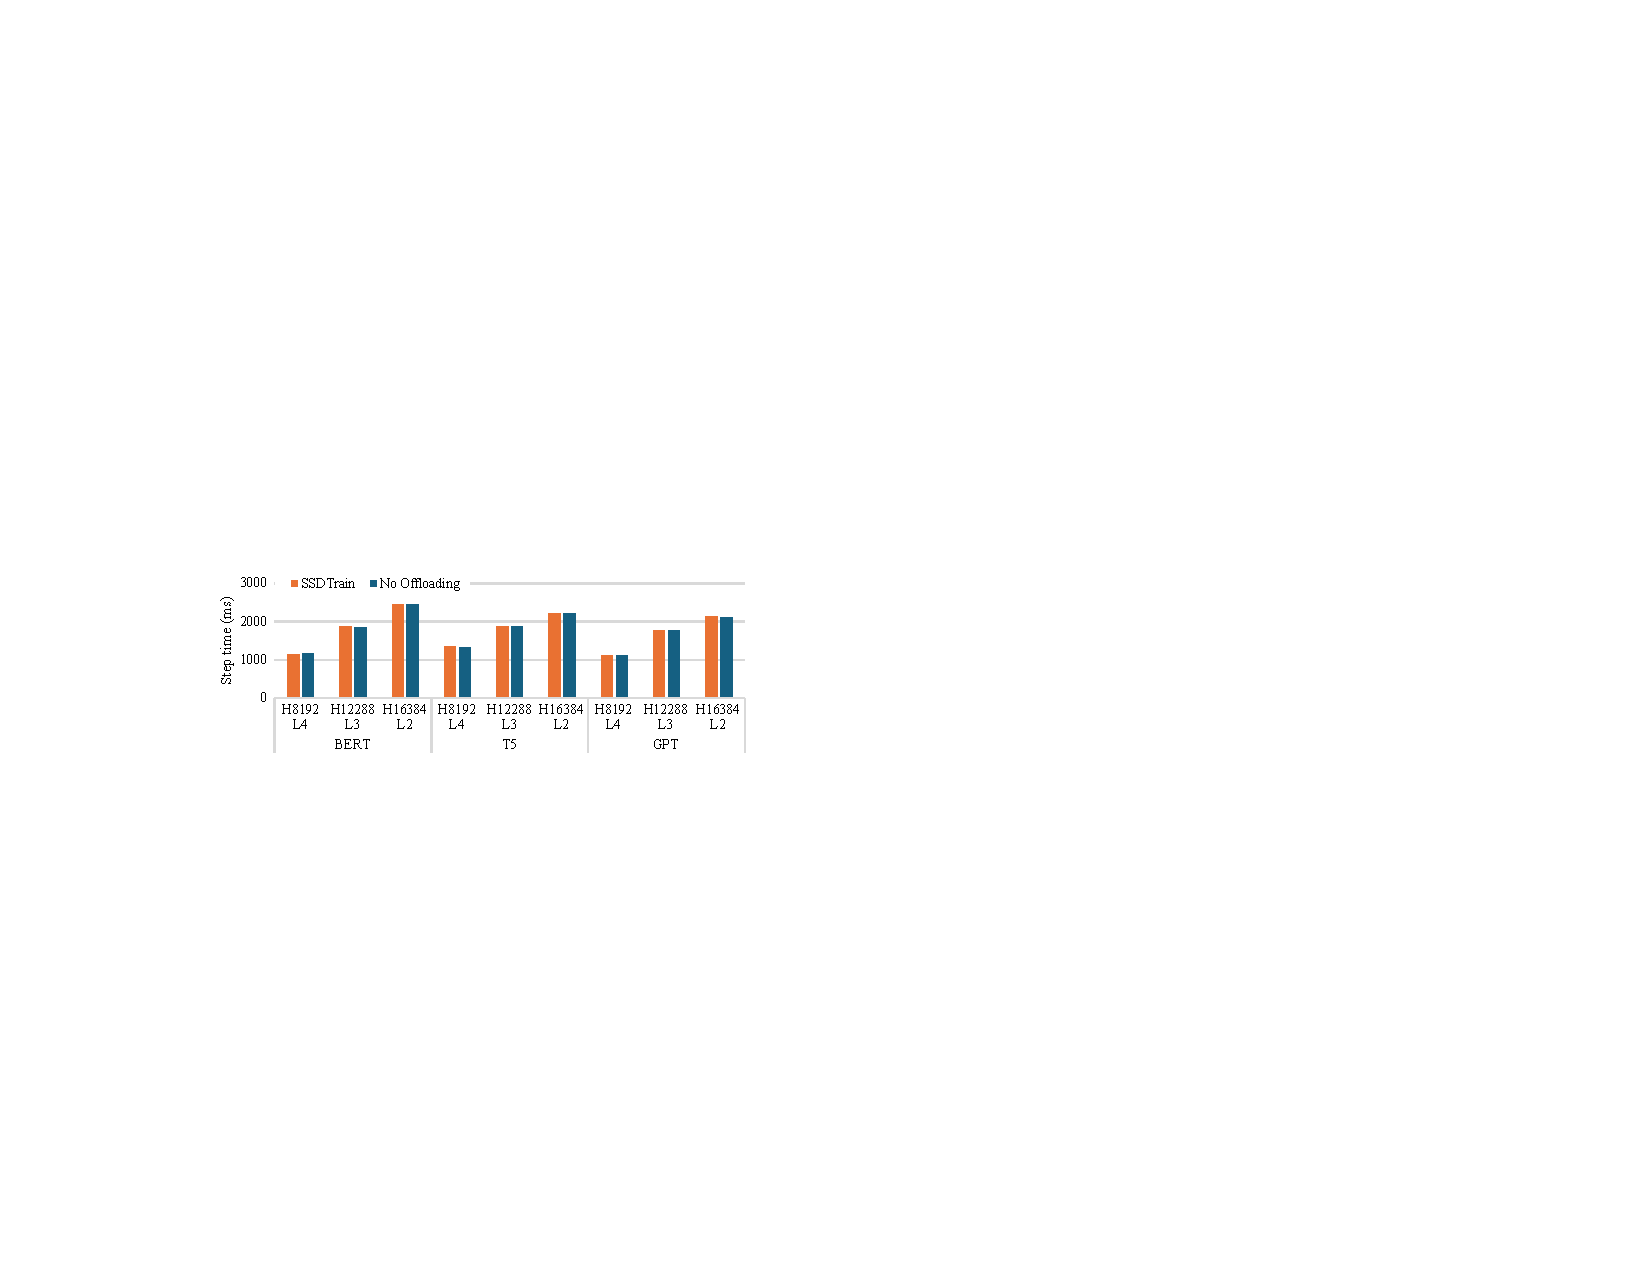
\includegraphics[scale=1.4]{figures/SSDTrain/eval_perf_a.pdf}}
\subcaptionbox{}
[\linewidth]{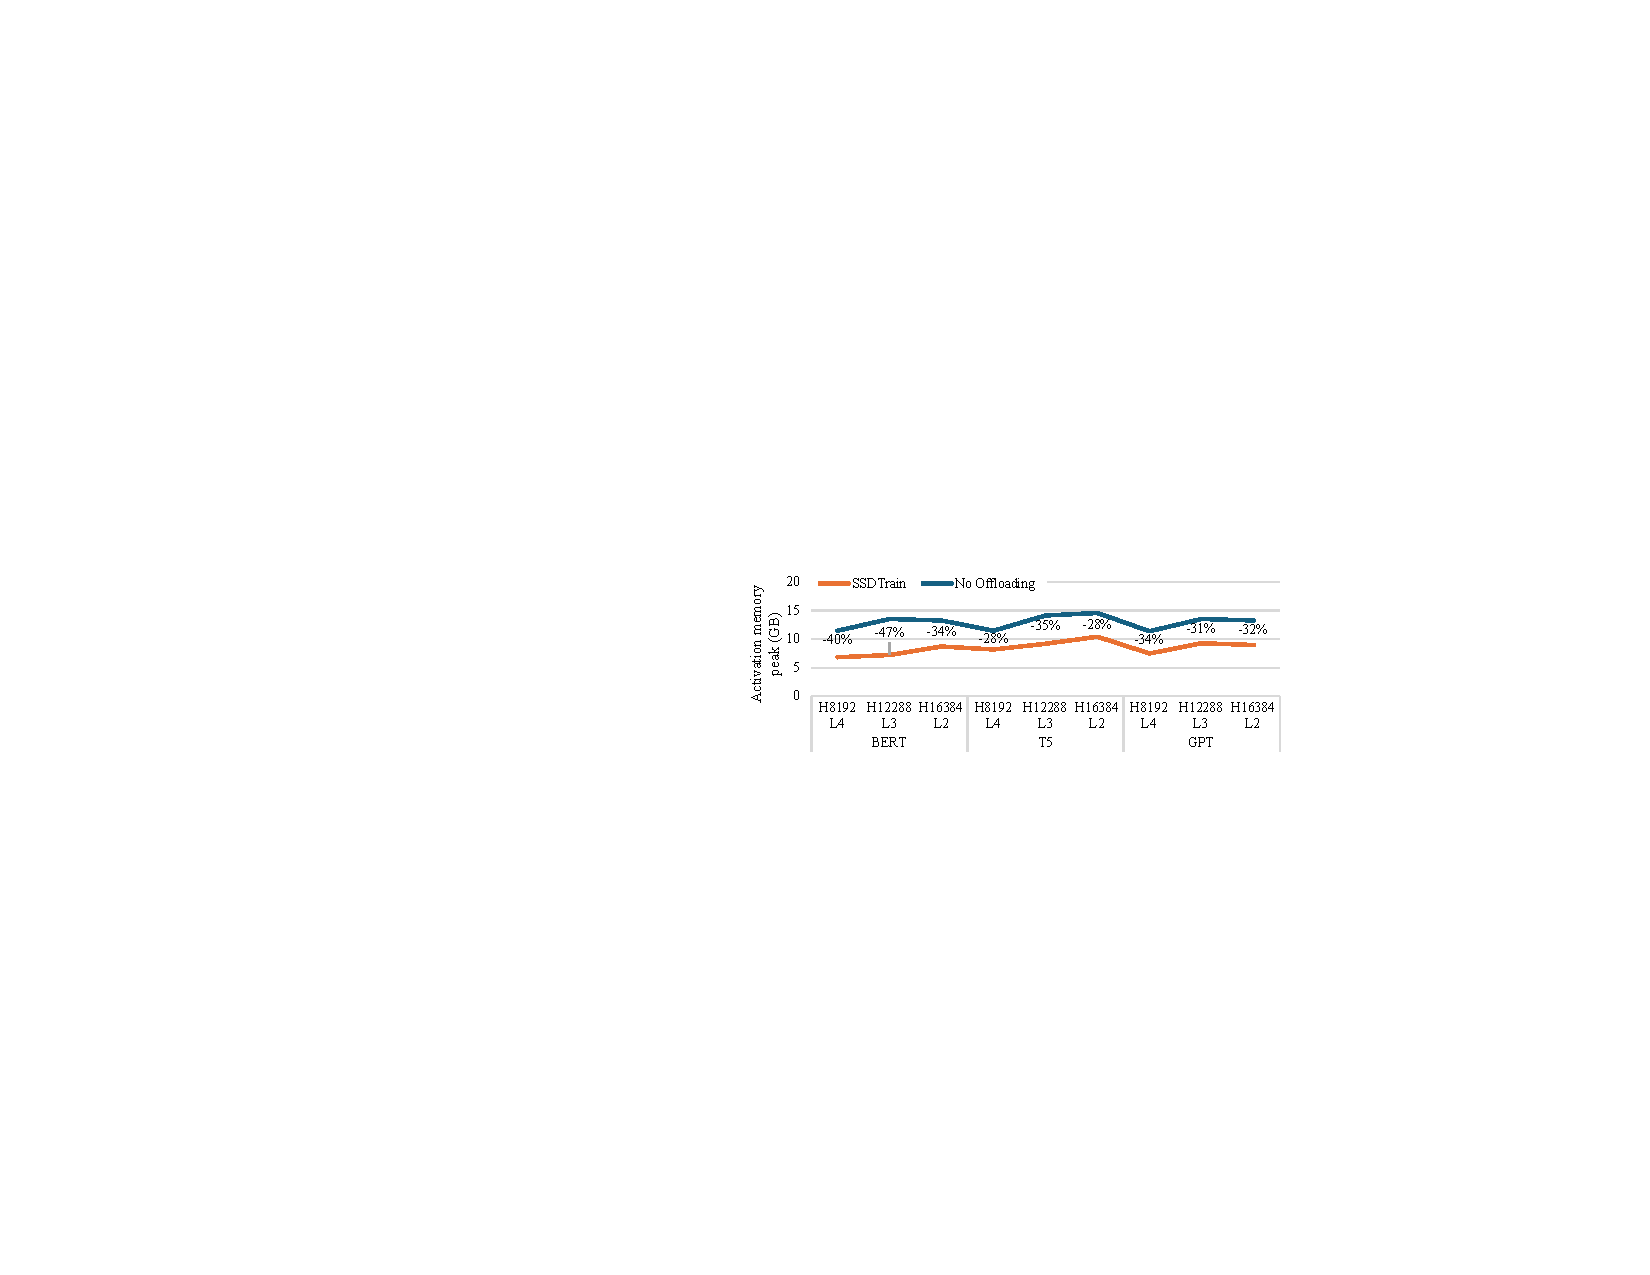
\includegraphics[scale=1.4]{figures/SSDTrain/eval_perf_b.pdf}}
\caption{\label{fig:eval_perf} Comparing the step time and activations memory usage of SSDTrain with execution without tensor offloading. We test several model configurations with different hidden dimensions~(H) and number of layers~(L). Global batch size is 16.}
\end{figure}



\subsection{Comparing the Activations Placement Strategies via Recompute-Offload-Keep~(ROK) Curve}
\label{sec:exp_dse}


SSDTrain opens up offloading activations to SSDs as an option besides keeping activations in the GPU memory and activations checkpointing. We compare the three strategies here by plotting the runs on the recompute-offload-keep~(ROK) curve.  
Figure~\ref{fig:eval_dse} shows the ROK curve for training two 3-layer BERT models, one with a hidden dimension of 12,288 and the other with a hidden dimension of 14,336. In a ROK curve, each training run is represented by a point. The x-axis is the activations memory peak, and the y-axis is the model throughput. Model throughput~\cite{shoeybiMegatronLMTrainingMultiBillion2020a} refers to the number of algorithmic computations \kwc{done in unit time} regardless of software and hardware implementation, e.g., whether the activations are recomputed.
In these two cases, SSDTrain reduces the GPU activations memory peak, allowing a larger micro-batch size to attain higher throughput. Given the same micro-batch size, SSDTrain offloading attains the throughput the same as the throughput when the activations are kept in memory. Meanwhile, SSDTrain gets a lower activations memory peak than the recomputation. Compared with keeping the activations in memory, SSDTrain can double the micro-batch size with the same activations memory budget. Alternatively, people could leverage SSDTrain to run a bigger model or use fewer GPUs.



Other than the three strategies, before FlashAttention~\cite{daoFlashAttentionFastMemoryEfficient2022}, Megatron~\cite{korthikantiReducingActivationRecomputation2022} proposed selective recomputation:
noting that in the transformer layer, the operations performed by the core attention module~(the whole gray box in Figure~\ref{fig:transformer}) require less computation but create a large intermediate tensor when compared with the MLP block, the work recomputed only the core attention module.
As we adopt FlashAttention, the core attention module is done in one kernel, eliminating these intermediate tensors.  The effect of selective recomputation with FlashAttention has a negligible impact on the performance and the peak memory usage for activations.



\begin{figure}[!htbp]
\centering
\subcaptionbox{H12288 L3}
[\linewidth]{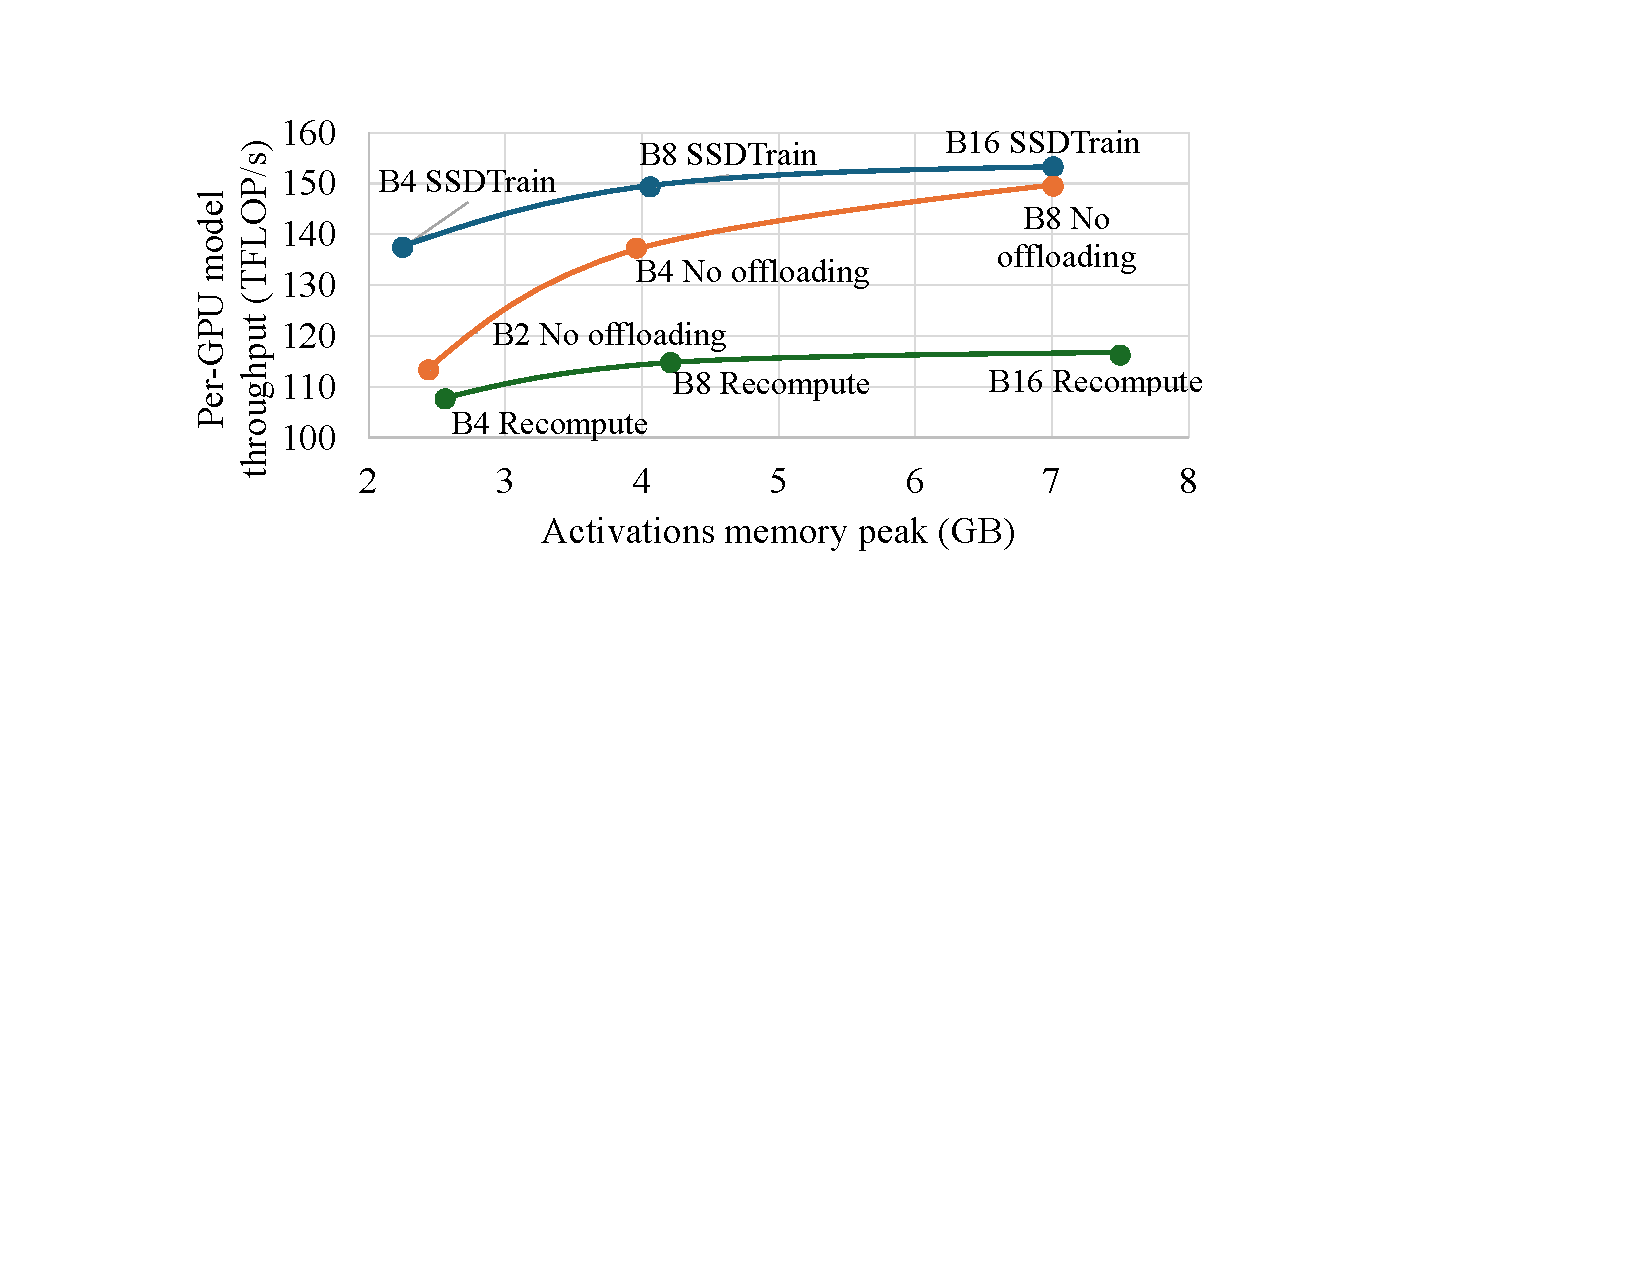
\includegraphics[scale=0.7]{figures/SSDTrain/eval_dse_a_v2.pdf}}
\subcaptionbox{H14336 L3}
[\linewidth]{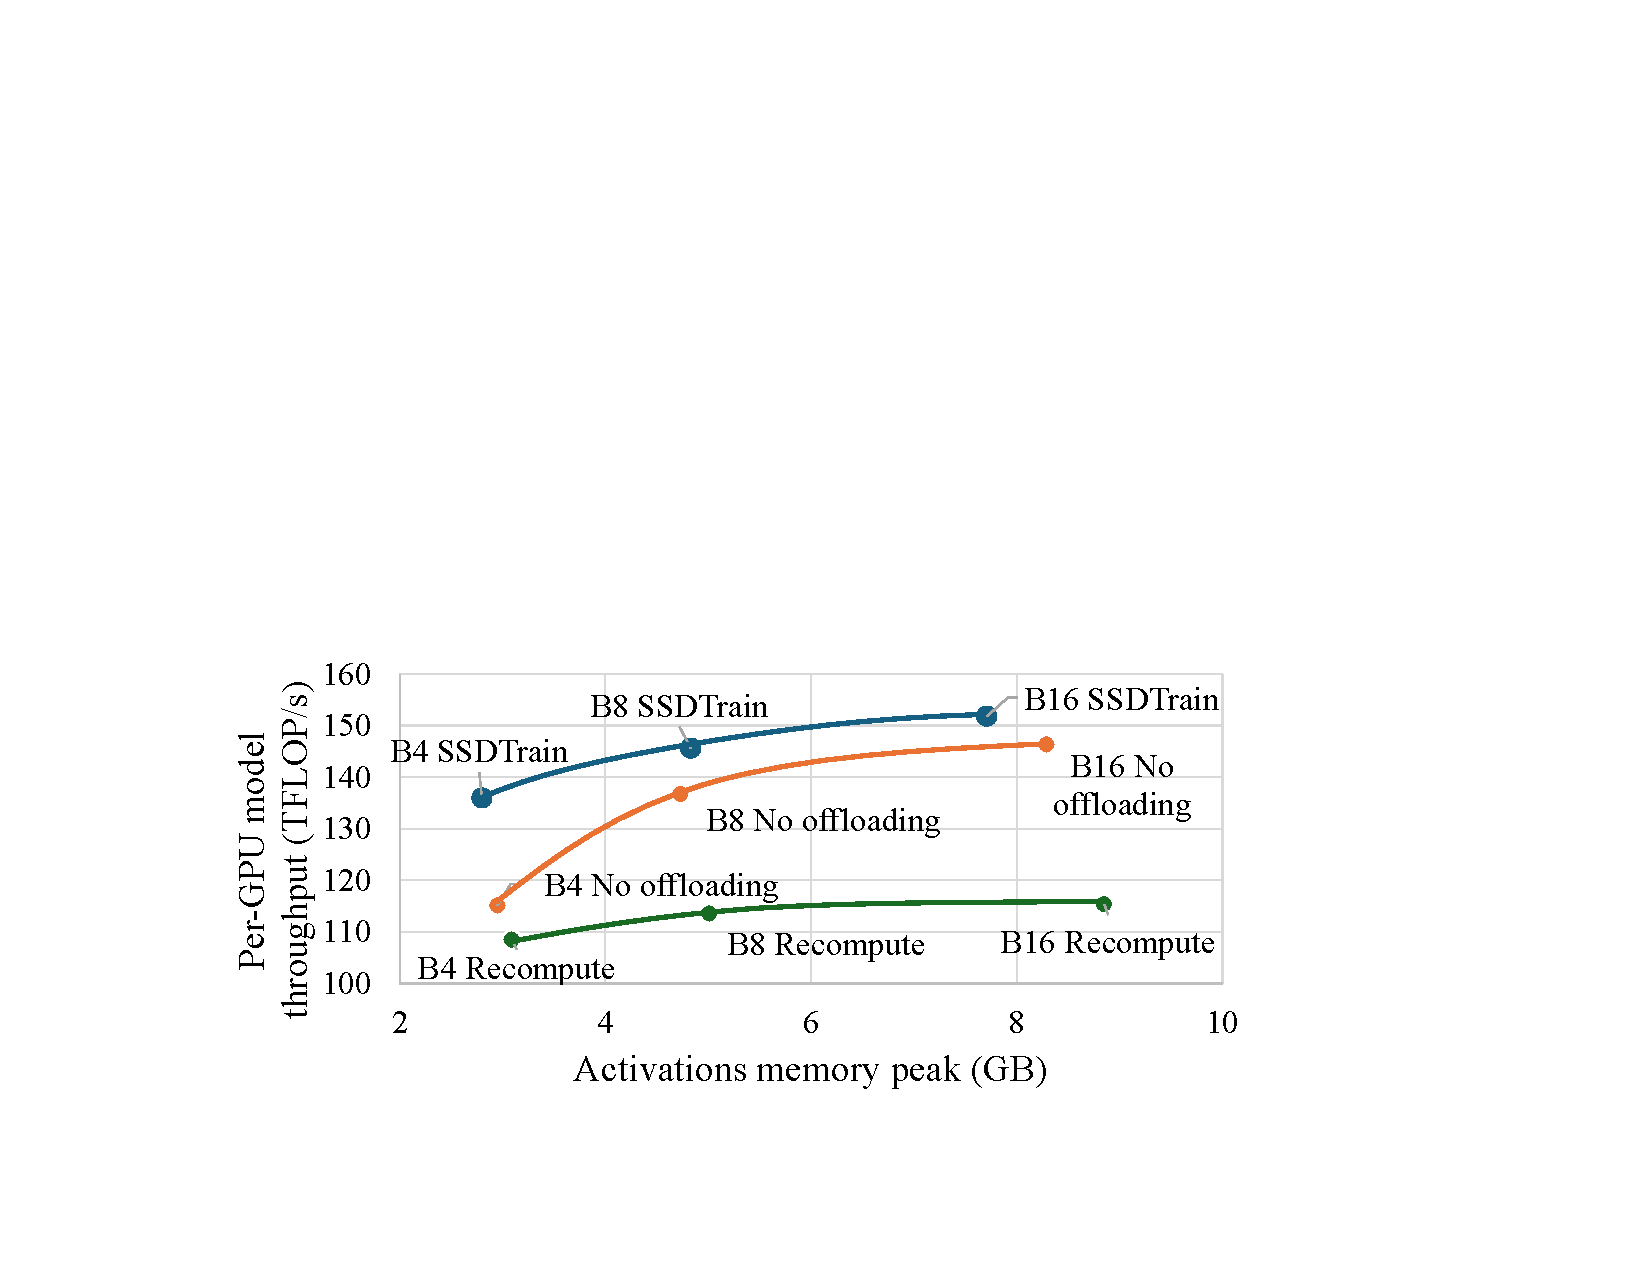
\includegraphics[scale=0.7]{figures/SSDTrain/eval_dse_b_v2.pdf}}
\caption{\label{fig:eval_dse}Recompute-offload-keep~(ROK) curve of BERT with 3 layers~(L) and hidden dimension~(H) as \textbf{(a)} 12,288 or \textbf{(b)} 14,436. Designs with a combination of \kwc{global} batch sizes~(B) and choices to offload activations, keep activations, or recompute activations are shown. \kwa{(Figure updated.)}}
\end{figure}




\subsection{Discussion}
\label{sec:discussion}
\subsubsection{Examining the Modeling}
To understand the accuracy of the performance model in Section~\ref{sec:projected_life}, we compare the offloaded amount by SSDTrain with the model estimate. As shown in Table~\ref{tab:eval_activations}, the figures are close. We also compute the required PCIe write bandwidth using half of the measured training time. The PCIe write bandwidth is reduced as the hidden dimension gets larger. Typically, a model with more than 60B parameters has a hidden dimension of no less than 8K~\cite{touvronLlamaOpenFoundation2023,jordanhoffmannTrainingComputeOptimalLarge2022}. The PCIe write bandwidth of the BERT models aligns with the estimate in Section~\ref{sec:projected_life}.



\begin{table}[!htbp]
\centering
\begin{tabular}{llll}
\toprule
                              & H8192 L4  & H12288 L3 & H16384 L2 \\\midrule
\textbf{Offloaded amount}     & 10.37 GB  & 12.85 GB  & 10.75 GB  \\
\textbf{Model estimate}       & 11.13 GB  & 12.60 GB   & 11.50 GB   \\
\textbf{PCIe write bandwidth} & 18.0 GB/s & 13.8 GB/s & 8.76 GB/s \\ \bottomrule
\end{tabular}
\caption{The per-GPU offloaded tensor amount and model estimate when running BERT with different hidden dimensions~(H) and number of layers~(L). The global batch size is 16. We also compute the per-GPU PCIe write bandwidth required to fully offload the tensors. \label{tab:eval_activations}}
\end{table}

\subsubsection{Impact of Upscaling} 
When LLM systems scale up, the computation efficiency decreases due to more cross-node communication.
Section~\ref{sec:llm_scaling} demonstrates that the whole-system activations size $S_{activations}$ grows slower than the whole-system GPU throughput $C$, i.e., $S_{activations} \propto C^{\frac{5}{6}}$. Therefore, the bandwidth required to fully overlap the computation with the SSD accesses is reduced.
In short, LLM scaling is essentially a weak scaling scenario, and SSD I/O latency is easier to hide when scaled up. 

\kwc{As shown in Table~\ref{tab:eval_activations}, the required SSD throughput per GPU to fully offload tensors is negatively correlated with the hidden dimension of the LLM model, a factor of the model scale. Since most computation is GEMM, theoretically, the required SSD throughput per GPU is approximately inversely proportional to the hidden dimension of the LLM model, assuming the GPU model and computational efficiency are the same. The evaluation shows that the SSDTrain offloading performs well with two GPUs and a hidden dimension of 8K. Given that all data transfers SSDTrain offloading incurs are within the node, this configuration pressured the system more than some larger configurations, e.g., four GPUs per node and hidden dimension as 16K.

In Table~\ref{tab:upscaling_write_bandwidth}, we further project the impact of upscaling on the write bandwidth per GPU using \texttt{llm-analysis}. We follow typical parallelism configurations~\cite{shoeybiMegatronLMTrainingMultiBillion2020a,nitinScalingLargeLanguage2023} when the number of GPUs is less than 100: Initially, all GPUs are dedicated to tensor parallelism, and as the number of GPUs increases, we gradually increase the pipeline parallelism factor. In all projected cases, the write bandwidth per GPU is smaller than the corresponding original two-GPU case shown in Table~\ref{tab:eval_activations}. Notice that Table~\ref{tab:upscaling_write_bandwidth} does not study the effect of data parallelism, which is typically adopted when the number of GPUs exceeds 100. Vanilla data parallelism only affects the weight update stage and does not affect the write bandwidth because SSD offloading and reloading only happen during forward and backward propagation. A configuration with ZeRO-enabled data parallelism has no greater required write bandwidth than the corresponding configuration without data parallelism because the introduced communication operations may delay forward propagation and backward propagation.



}

\begin{table}[!htbp]
\begin{subtable}[]{\textwidth}\centering
\begin{tabular}{lrrrrr}\toprule
\textbf{Number of layers}                          & 4    & 4    & 8    & 16   & 32   \\
\textbf{Tensor   parallelism factor}               & 4    & 8    & 8    & 8    & 8    \\
\textbf{Pipeline   parallelism factor}             & 1    & 1    & 2    & 4    & 8    \\\midrule
\textbf{Write bandwidth per GPU (GB/s)}  & 17.3 & 16.0 & 16.5 & 16.8 & 17.0 \\
\bottomrule
\end{tabular}
\caption{Hidden dimension as 8,192. In all cases, the required write bandwidth per GPU is smaller than the original case's 18.0 GB/s.}
\end{subtable}\vspace{0.3cm}


\begin{subtable}[]{\textwidth}\centering
\begin{tabular}{lrrrrr}\toprule
\textbf{Number of layers}                          & 3    & 3    & 6    & 12   & 24   \\
\textbf{Tensor   parallelism factor}               & 4    & 8    & 8    & 8    & 8    \\
\textbf{Pipeline   parallelism factor}             & 1    & 1    & 2    & 4    & 8    \\\midrule
\textbf{Write bandwidth per GPU (GB/s)}  & 13.4 & 12.7 & 13.1 & 13.3 & 13.4 \\
\bottomrule
\end{tabular}
\caption{Hidden dimension as 12,288. In all cases, the required write bandwidth per GPU is smaller than the original case's 13.8 GB/s.}
\end{subtable}\vspace{0.3cm}


\begin{subtable}[]{\textwidth}\centering
\begin{tabular}{lrrrrr}\toprule
\textbf{Number of layers}                          & 2    & 2    & 4    & 8   & 16   \\
\textbf{Tensor   parallelism factor}               & 4    & 8    & 8    & 8    & 8    \\
\textbf{Pipeline   parallelism factor}             & 1    & 1    & 2    & 4    & 8    \\\midrule
\textbf{Write bandwidth per GPU (GB/s)}  & 8.55 & 8.17 & 8.47 & 8.63 & 8.69 \\
\bottomrule
\end{tabular}
\caption{Hidden dimension as 16,384. In all cases, the required write bandwidth per GPU is smaller than the original case's 8.76 GB/s.}
\end{subtable}

\caption{Projecting the SSD write bandwidth required by each A100 when scaling up the cases shown in Table~\ref{tab:eval_activations}. As the number of GPUs increases, we first increase the tensor parallelism factor with the number of layers unchanged. Then, we increase the pipeline parallelism and increase the number of layers proportionally. \kwa{(New table.)} \label{tab:upscaling_write_bandwidth}}
\end{table}




\kwc{\subsubsection{Performance Implications of Larger Micro-Batch} To further understand how larger micro-batch size improves the performance, we compare the no-offloading cases in Figure~\ref{fig:eval_dse}(a) to the same configurations with global batch size as one and break down the throughput improvement in Table~\ref{tab:break_down_batch_effect}. The improvement comes from higher kernel throughput and time-saving by weight update, where weight update saving is consistently the primary source. Such a benefit is very relevant to large-scale LLM training systems. The micro-batch size is usually set as one or two in Paxml~\cite{googlePaxmlAkaPax2022} and BLOOM~\cite{workshopBLOOM176BParameterOpenAccess2023} pretraining. For these two models, the micro-batch size is set small in exchange for smaller bubbles introduced by the pipeline parallelism. The bubble time percentage is inversely proportional to the number of micro-batches. For example, in the BLOOM training system, the tensor parallelism factor is four, and the pipeline parallelism factor is 12. In each training step, each data-parallel rank is assigned a mini-batch with 32 samples. When the micro-batch size is no less than four, the ideal pipeline bubble time percentage is no less than 11.5\%. However, the weight update and gradient accumulation cost is inversely proportional to the micro-batch size. When the micro-batch size is one or two, the cost is enormous. SSDTrain allows larger micro-batch sizes given the same activation memory budget, thus beneficial to these pipeline-parallelism-enabled training systems. 

}

\begin{table}[]\centering
\begin{tabular}{lllll}
\toprule
\textbf{Global batch size}                   & 2      & 4      & 8      & 16     \\\midrule
\textbf{Throughput improvement}       & 27.6\% & 52.2\% & 66.1\% & 71.8\% \\
\textbf{By higher compute efficiency} & 10.5\% & 21.8\% & 27.7\% & 29.4\% \\
\textbf{By weight update saving}            & 17.1\% & 30.4\% & 38.4\% & 42.4\% \\\bottomrule
\end{tabular}
\caption{Breakdown of model throughput improvements for a three-layer BERT model with a hidden dimension of 12,288, compared to a baseline with global batch size as one. \kwa{(New table.)}}
\label{tab:break_down_batch_effect}
\end{table}

\kwc{\subsubsection{Weight Offloading}

This work focuses on offloading activations. When the size of weights gets larger, it becomes more desirable to offload weights. SSDTrain can be configured to offload weights as well. As Section~\ref{sec:tensor_cache} explained, the tensor cache keeps a record of all the weights and ignores them when the pack hook is triggered. The tensor cache may be modified to offload weights in a profitable situation. For each operator, e.g., a matrix multiply, the amount of computation, weight size, and input size can be determined from the model specification without execution. SSDTrain can decide whether to offload one or both according to the GPU FP16 throughput and SSD write bandwidth. A reasonable starting strategy is to offload as much as possible while staying within SSD write bandwidth. 

Furthermore, SSDTrain could be extended to generate an optimized plan for all operators in the model before the execution by framing the decision-making process into an optimization problem and solving it. Offloading weights works when the pipeline parallelism factor is small. When the pipeline parallelism factor is large, careful planning is needed to determine what to offload because some weights are immediately reused by the later micro-batches.

Notice that offloading weights to the main memory, together with weight update to the CPU, has been explored in prior work~\cite{rajbhandariZeROinfinityBreakingGPU2021,kamahoriFiddlerCPUGPUOrchestration2024}. In the future, it may be explored to use SSDTrain together with any of the prior work to offload activations to the device memory and offload weights to the main memory. We leave the discussion to the elaboration on \textbf{Swapping and offloading} in Section~\ref{sec:ssdtrain_related}.


}


\subsubsection{Cost Analysis} We study the SSD cost associated with adopting SSDTrain offloading in LLM systems.
To obtain the endurance in Figure~\ref{fig:projected_perf_model}, each A100 priced at US\$10K~\cite{dihuniNVIDIAA1009002100100000002021} is paired with a total of US\$6.4K worth of SSDs.
In the evaluation, we allocate seven Intel Optane P5800X for the two A100s. Although P5800X is more expensive than the models in Table~\ref{tab:ssd}, the price per PBW is comparable at US\$10.27~\cite{neweggIntelOptaneDC2021}.
We can further reduce the cost to a few percentage points by relaxing the data retention period: \kwc{For example, for all cases shown in Figure~\ref{fig:projected_perf_model}, Figure~\ref{fig:projected_endurance_980pro_1TB} shows that using four Samsung 980 PRO 1 TB for each A100 provides more than two years of SSD lifespan. The corresponding SSD cost is US\$360 per A100}~\cite{samsungSamsungVNANDSSD2021,bestbuySamsung980PRO2022}.
To have more durable storage for other data, the system may restrict the activation offloading to dedicated SSDs or utilize hardware equipped with Zoned Namespaces~(ZNS) standard~\cite{stavrinosDonBeBlockhead2021,hanZNSAdvancedZoned2021} to confine the wear within designated zones of physical blocks on the same SSD.

\kwc{Another significant cost factor is electricity. Each SSD costs around 20 watts, whereas a single GPU can easily draw several hundred watts. Taking other factors, e.g., commissioning, cooling, etc., into consideration~\cite{barrosoDatacenterComputerDesigning2019,redoakconsultingTotalCostOwnership2024}, the total cost of ownership~(TCO) of each GPU is an order of magnitude higher than its corresponding SSDs~\cite{dylanpatelNvidiaBlackwellPerf2024,sniaSNIAEnterpriseTCO2020}.}

\kwc{\subsubsection{Future Viability}
Will NVMe SSDs continue to be a good offloading target in the future? As shown in Figure~\ref{fig:gpu_trend_various}, historically, the PCIe bandwidth per lane has grown faster than the minimum requirement to keep up with the FP16 throughput, i.e., $\frac{5}{6}$ of the growth rate of FP16 throughput. The PCIe bandwidth has continued to grow rapidly, with new standards frequently released that double the bandwidth per lane of the previous version. 
Whenever a new PCIe standard is adopted, SSD vendors promptly release SSD products that provide the increased bandwidth aligned with the new PCIe standard. 
Therefore, the analysis we have done and all the conclusions we have drawn on SSDs in Chapter~\ref{ch:ssdtrain} will still be valid in the future.
}



\kwc{\subsubsection{Bringing It Altogether: System Design Decisions}


First, \textbf{Cost Analysis} shows the cost of SSDs in a system with SSDTrain enabled is an order of magnitude lower than that of GPUs. Therefore, adopting SSDs to enable SSDTrain, whether as an upgrade to existing on-premises clusters or in new on-premises machines, is profitable. The power supply should not be a problem: Typically, clusters have sufficient power redundancy to support upgrades that add new SSDs~\cite{barrosoDatacenterComputerDesigning2019}. However, adopting SSDs in cloud instances may not be profitable if high-throughput SSDs are too costly~\cite{googleGoogleCloudHyperdisk}.

Second, some clusters may have a lower \kwc{SSD-to-GPU} ratio.  
Two measures can be taken for such clusters. First, a portion of the processes on the node can use the CPU offloader (Figure~\ref{fig:software_arch}) to offload tensors to the CPUs. Second, the adaptive offloading mechanism (Figure~\ref{fig:adaptive}) measures the I/O bandwidth and determines the amount of tensors to be offloaded so as not to delay the training process. 

Let us conduct a case study on DGX H100 systems~\cite{nvidiaIntroductionNVIDIADGX2023}. Each DGX H100 node is equipped with dual-socket CPUs and eight GPUs. Within each DGX H100 node, in addition to 10 local NVMe SSDs, a significant number of PCIe lanes are allocated to storage network adapters that enable high-performance access to NVMe over Fabrics (NVMe-oF)~\cite{nvmexpressinc.NVMExpressMoves2016}. Since GDS supports both local NVMe SSDs and remote NVMe-oF SSDs, SSDTrain is compatible with both types of storage in the DGX H100 system. GDS still provides acceleration~\cite{handwikiSoftwareLustreFile2021,raviGPUDirectHDF52020} when the remote SSDs are purposed as a distributed file system, e.g., Lustre, and optimized file format is used, e.g., HDF5. Users can choose to offload activations to local SSDs when their bandwidth and capacity are sufficient. If additional bandwidth or capacity are needed, users may utilize remote SSDs when available and/or choose the host memory as an additional target, as discussed above.

}

\begin{figure}[!t]
\centering
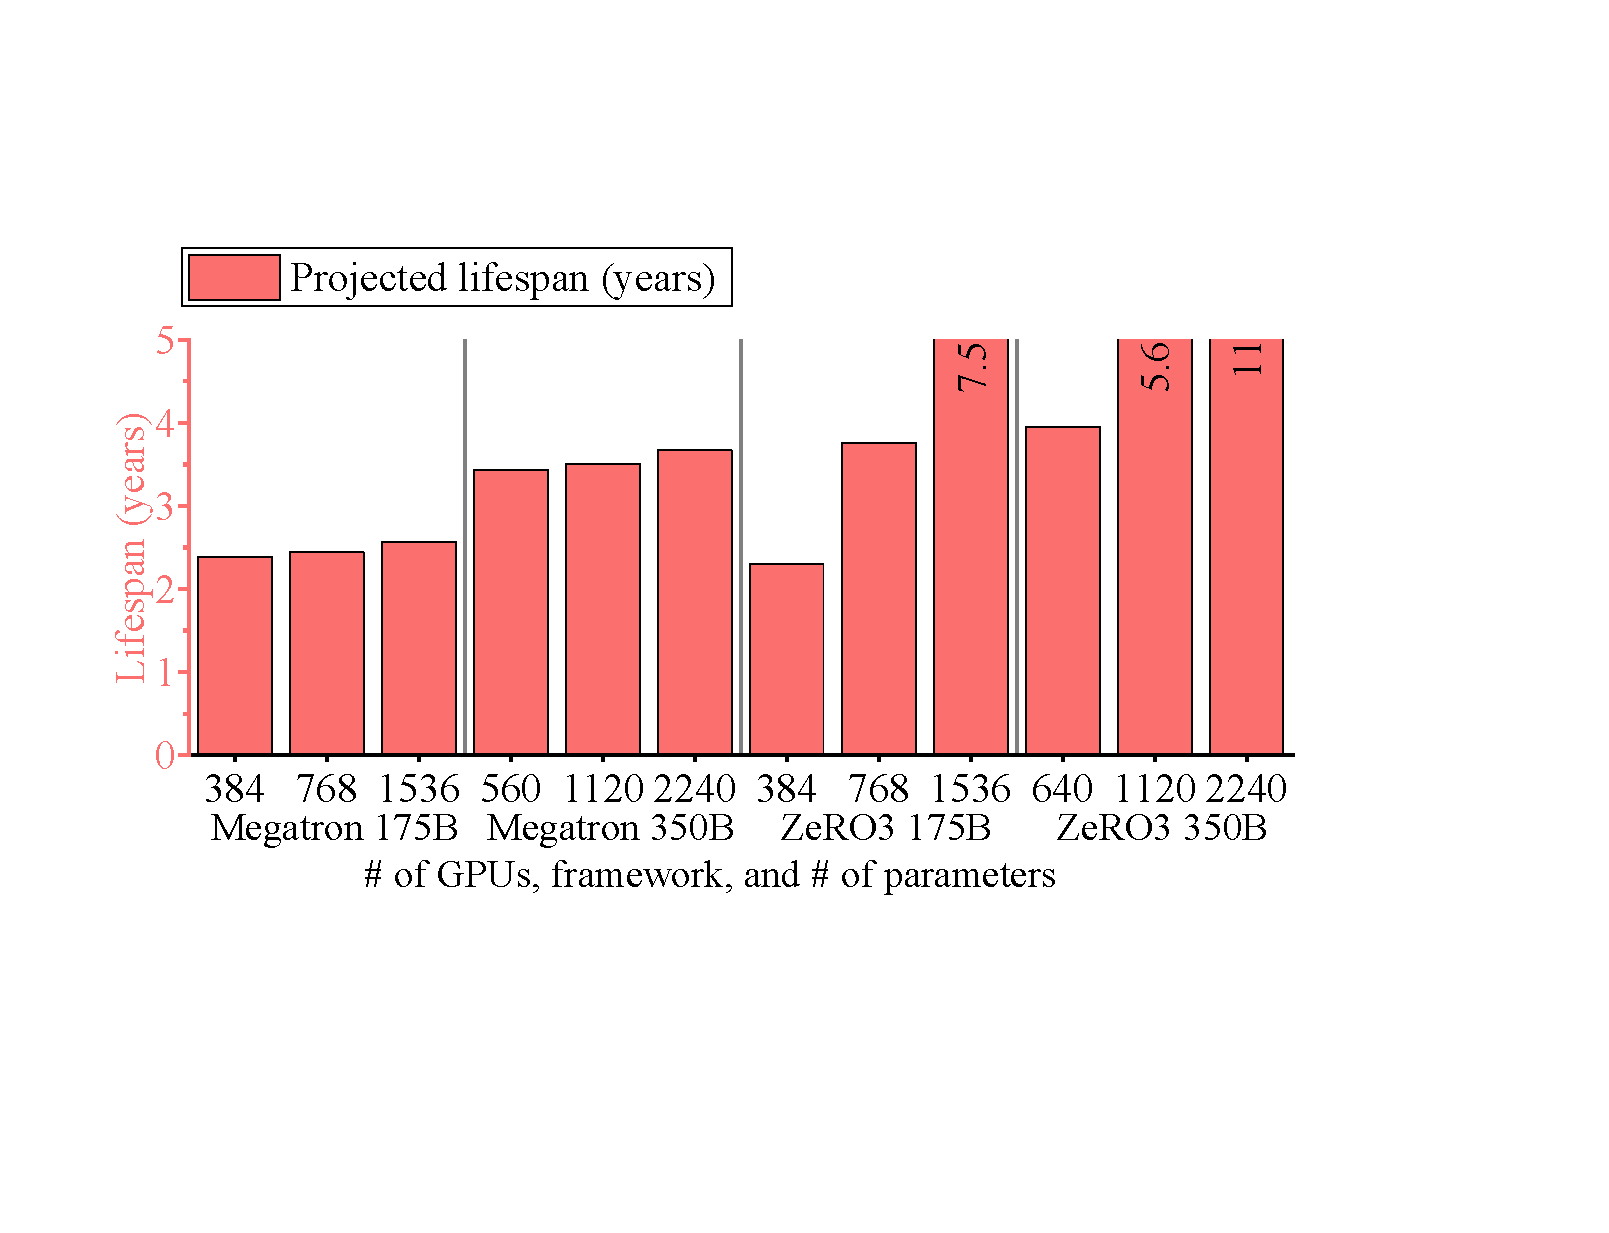
\includegraphics[width=0.95\linewidth]{figures/SSDTrain/ProjectedPerfModel3_980pro_1TB_endurance.pdf.pdf}
\caption{\label{fig:projected_endurance_980pro_1TB} \kwc{Estimate of SSD lifespan in scenarios of Figure~\ref{fig:projected_perf_model} with the assumption that each A100 is paired with four Samsung 980 PRO 1TB.}}
\end{figure}
